\section{SGLD in Actor-Critic}
Under the Bayesian learning framework, there is one mathematical method that has both the "posterior sampling" and "parameter noise" properties, called stochastic gradient Langevin dynamics. In this section, we will briefly introduce the SGLD and show how it can be used to construct an exploration strategy in Actor-Critic algorithms.

\subsection{Stochastic Gradient Langevin Dynamic}
Stochastic Gradient Langevin Dynamic algorithm is an algorithm that can perform MCMC sampling by stochastic gradient descent + Gaussian noise \cite{SGLD}. For a paramter vector $\theta$ with a prior distribution $p(\theta)$ ,to draw a sample chain $\{\theta_1,\theta_2,\cdots\}$ follow $p(\theta|D)$ where $D=\{d_i\}^N_{i=1}$, the parameters should be updated as follow:
\begin{equation}
   \label{eq:sgld} 
   \begin{aligned}
\Delta\theta =\frac{\epsilon}{2}\frac{N}{n}\sum_{i=1}^{n}\nabla_\theta\log p(d_i|\theta)+\frac{\epsilon}{2}\nabla_\theta\log p(\theta)\\
+\mathcal{N}(0,\epsilon)
\end{aligned}
\end{equation}
Where $\epsilon$ is the learning rate, $n$ is the size of one mini-batch. 

The basic SGLD algorithm updates all parameters with the same step size, which leads to slow mixing rate. In practical, we use preconditioned SGLD (pSGLD) instead, in which the step size is scaled by preconditioner $G_t$ as follow:
\begin{equation}
   \label{eq:psgld} 
   \begin{aligned}
      \Delta\theta =\frac{\epsilon}{2}\frac{N}{n}G_t\sum_{i=1}^{n}\nabla_\theta\log p(d_i|\theta)+\frac{\epsilon}{2}G_t\nabla_\theta\log p(\theta)\\
      +\mathcal{N}(0,\epsilon G_t)
   \end{aligned}
\end{equation}
Where $G_t$ is updated as the mean square term in RMSprop \cite{rmsprop}.
\begin{figure*}[htbp]
   \begin{center}
      \centerline{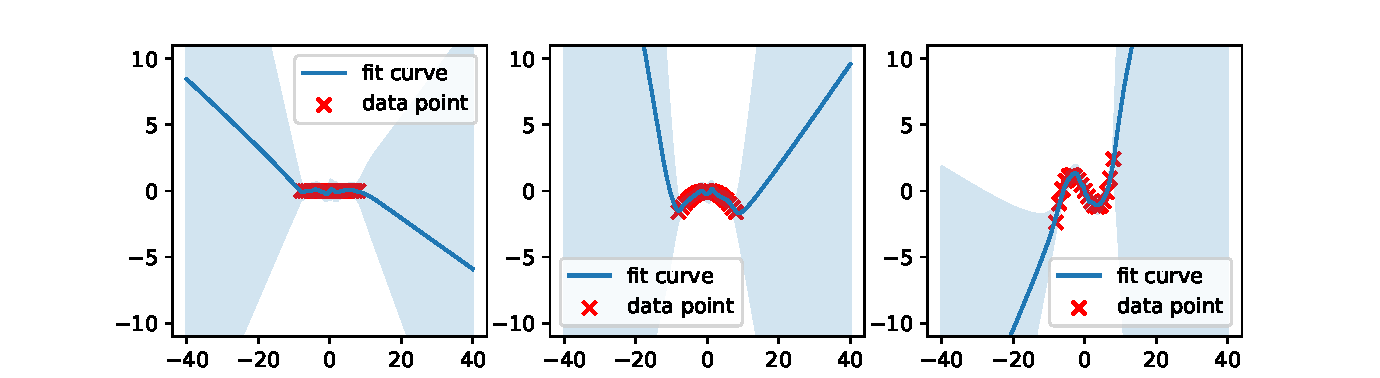
\includegraphics[width=480pt]{figs/three-curve}}
   \caption{The results of curve fitting by using pSGLD on three toy data sets.}
   \label{fig:three}
   \end{center}
\end{figure*}

%$\nabla_\theta p(d_i|\theta)$ is the data like-hood term, which corresponding to gradient of loss. $\nabla_\theta p(\theta)$ is prior probability term, it is equivalent to L2 regularization if $p(\theta)\sim\mathcal{N}(0,\sigma^2)$. And $\mathcal{N}(0,\epsilon)$ term make SGLD can sample parameters with $\theta \sim p(\theta|D)$
To visualize the ability of pSGLD to characterization the uncertainty of posterior distribution when fitting data set, we trained a neural network with architecture of "20-ReLU-20-ReLU-1" by pSGLD on three toy datasets, left: $y=0$, mid: $y=-x^2$, right: $y=x^3-x$, and the results are shown in the figure \ref{fig:three}. The dark curve is the average of the curve clusters, and the light areas represent the standard deviation of the curve clusters. The results show that the curve samples of pSGLD are concentrated near the data points, while diverge in both positive and negative directions in areas far from the data, even on the all zero data set.

\subsection{Posterior sampling of critic}
\label{sec:samplecritic}
In Deep Actor Critic algorithm, the parameters of critic network $\theta^Q$ is updated by an SGD-like optimizer to minimize the MSE error $L^Q=\sum(R-V(S|\theta^Q))$. To replace the SGD-like optimizer by pSGLD sampler with minimal changes, we suppose that the likelihood term is $p(d_i|\theta^Q)\sim\exp(-L^Q)$ to match the Bellman error, and prior term is $p(\theta^Q)\sim \mathcal{N}(0,\sigma^2)$ to match the L2 regularization on critic network. Then the critic will updated as follow :
\begin{equation}
   \label{eq:rlpsgld} 
   \begin{aligned}
      \Delta\theta^Q =-\frac{\epsilon}{2}\frac{N}{n}G_t\sum_{i=1}^{n}\nabla_\theta L^Q -\frac{\epsilon}{2}G_t \frac{\theta^Q}{\sigma^2}\\
      +\mathcal{N}(0,\epsilon G_t)
   \end{aligned}
\end{equation}
It is worth noting that, for off-policy algorithm with replay buffer, the size of data sets $N$ in reinforcement learning is increasing as the training process increases. If the learning rate $\epsilon$ remains constant, the gradient of the likelihood term will continue to grow, resulting in an unstable training process. In order to keep the training process stable, we implement learning rate decay as opposed to data set size growth: $\epsilon_t=\frac{n}{N}\epsilon_0$. Now the equation (\ref{eq:rlpsgld}) turns into:
\begin{equation}
   \label{eq:rlpsgld1} 
   \begin{aligned}
      \Delta\theta^Q =-\frac{\epsilon_0}{2}G_t\sum_{i=1}^{n}\nabla_\theta L^Q -\frac{\epsilon_0}{2}\frac{n}{N}G_t \frac{\theta^Q}{\sigma^2}\\
      +\mathcal{N}(0,\epsilon_0\frac{n}{N} G_t)
   \end{aligned}
\end{equation}
The observed data is increasing as the learning process progresses, which leads to the effect of the prior term and the noise term becomes weaker than the likelihood term. This is consistent with our common sense: the more data is observed, the more the model's distribution is concentrated toward the maximum likelihood estimate.
\begin{algorithm}[htbp]
   \caption{Deep Actor Critic with SGLD}
   \label{alg:sgldac}
\begin{algorithmic}
   \STATE {\bfseries Input:} environment $E$, critic $V(s|\theta^V)$, actor $\pi(s|\theta^\pi)$, exploration strategy $\tilde\pi \leftarrow f(\pi)$
   \FOR{1 {\bfseries to} cycle\_number}
   \STATE Copy the actor for rollout $\tilde \pi\leftarrow \pi$
   \FOR{1 {\bfseries to} rollout\_update\_number}
   \STATE Update $\tilde\pi$ by policy gradient with last critic.
   \ENDFOR
   \STATE Rollout data $\{d_t\}$ from $E$ by $\tilde\pi$
   \FOR{1 {\bfseries to} update\_number}
   \STATE Sample Critic $V(s|\theta^V) \sim p(\theta^V|D)$ with SGLD
   \STATE Update Actor $\pi(s|\theta^\pi)$ by policy gradient 
   \ENDFOR
   \ENDFOR
\end{algorithmic}
\end{algorithm}
\subsection{Exploration for Actor-Critic Algorithm}
The Actor-Critic algorithm using SLGD is shown in algoritm \ref{alg:sgldac}. Critic $V(s|\theta^V)$ is continuously sampled by SGLD, so the last critic in the network is a sample follow $p(\theta^V|D)$ at any time. In the rollout phase, the current actor $\pi$ is copied to $\tilde\pi$, then update $\tilde\pi$ use the policy gradient generated by the last critic. In Actor-Critic algorithm, the critic does not make decisions directly, so we optimize the copy of current actor with the last critic sample to get the optimal strategy of the last critic. We do this to follow the principle of Thompson sampling: making decisions based on the sampled value prediction model. The policy gradient with posterior sampled critic can estimated follow equation \ref{eq:acpg}, which similar as \cite{dropoutInference}.
\begin{equation}
   \label{eq:acpg} 
   \begin{aligned}
   \nabla_{\theta^\pi}\mathbb{E}[L^\mu|D] = \mathbb{E}_{s_t\sim\rho,a_t\sim\pi,\theta^V\sim p(\theta^V|D)}[\nabla_{\theta^\pi}L^\pi]\\
   \end{aligned}
\end{equation}
Now we confirm the sanity check as \cite{osband2018randomized} one by one: \textbf{Posterior Concentration}: As described in section \ref{sec:samplecritic}, the intensity of the noise term and prior term will be weaker as more data is observed, and the distribution of critic will concentrate to the most likelihood estimation. \textbf{Multi-step Uncertainty}: The uncertainty of critic will be propagated throught the bootstrap value estimation target $R$. \textbf{Epistemic vs Aleatoric}: The SGLD sampler does posterior sampling follow $p(\theta^V|D)$ instead of $p(r_t|s_t,a_T)$. \textbf{Task-appropriate}: The SGLD sampler does posterior sampling in parameter space instead of state-action space which related to the environment. \textbf{Intrinsic motivation}: Even in zero reward environment, the SGLD sampler can give non-zero value estimation on unseen states. These analysis demonstrate that SGLD based exploration strategy can effectively overcome the shortcomings of existing exploration strategies.